\chapter{Case Study}
\todo{I don't like the name case study, since it is not really a study. What about initial evaluation? self evaluation? merge with previous chapter and make it a section?}

\todo{first general showcase from icra paper (does not have the plot widget in the screenshots), then how to add a new widget --> plot widget. Then the more specific audio source localization / sound localization showcase with nao}

\section{Visualizing Existing Data}
Although the current implementation is a prototype, it has all the features that were initially planned. The implementation is running stably and first attempts to use it as a debugging tool have been made. ROSDashboard is ready to be used for the development of robot applications and can be used for further evaluations (see Section~\ref{future_work}).

Figure~\ref{showcase} shows a simple showcase scenario: ROSDashboard is running alongside the \emph{turtlesim\_node} node which is used in many examples in the ROS tutorials\footnote{http://www.ros.org/wiki/ROS/Tutorials}. It monitors the values for linear and angular speed which are published by the \emph{turtle\_teleop\_key} node to control the turtle simulation. The String widget is configured to display messages from \emph{/rosout}, which in this example shows a warning when the turtle hits a wall.
For the purpose of this small showcase, there was no need to modify the turtlesim source code. The only topics used by the showcase scenario are topics that are already used to control the turtle in the simulation and to display warnings.

\begin{figure}[thpb]
  \centering
  \framebox{
    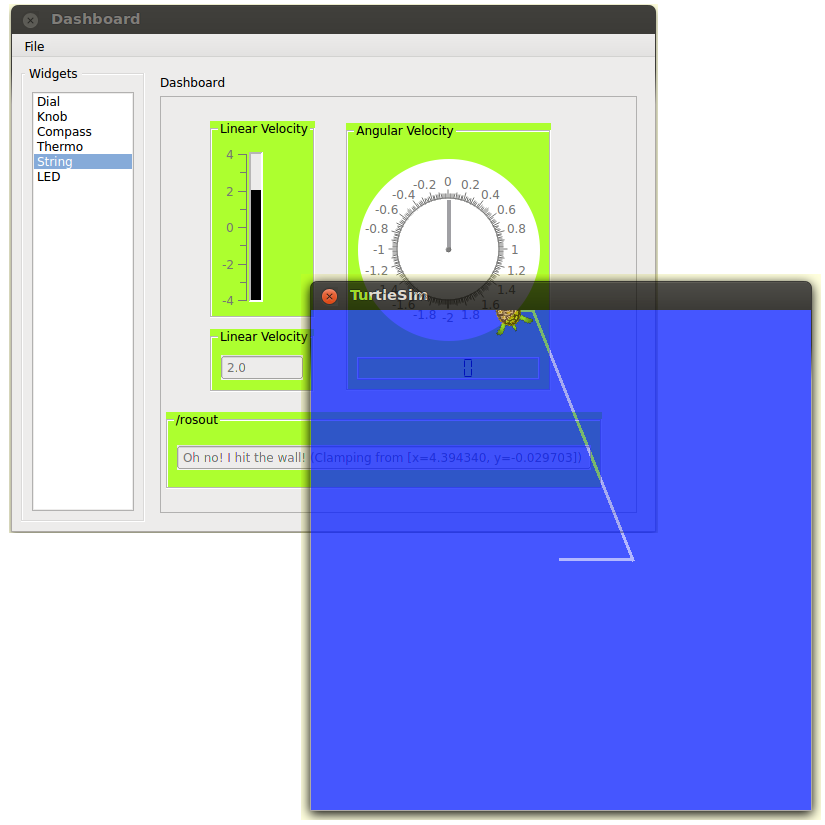
\includegraphics[width=0.9\textwidth]{img/showcase3.png}
  }  
  \caption{ROSDashboard running alongside turtlesim\_node.}
  \label{showcase}
\end{figure}

Figure~\ref{rosgraph_simple} shows the ROS computation graph during the execution of the showcase scenario. It shows how ROSDashboard is connected to the nodes which are debugged. The topics needed for the showcase are \emph{/turtle1/command\_velocity} for the linear and angular velocity and \emph{/rosout} for warnings when the turtle hit the wall.

\begin{figure}[thpb]
  \centering
  \framebox{
    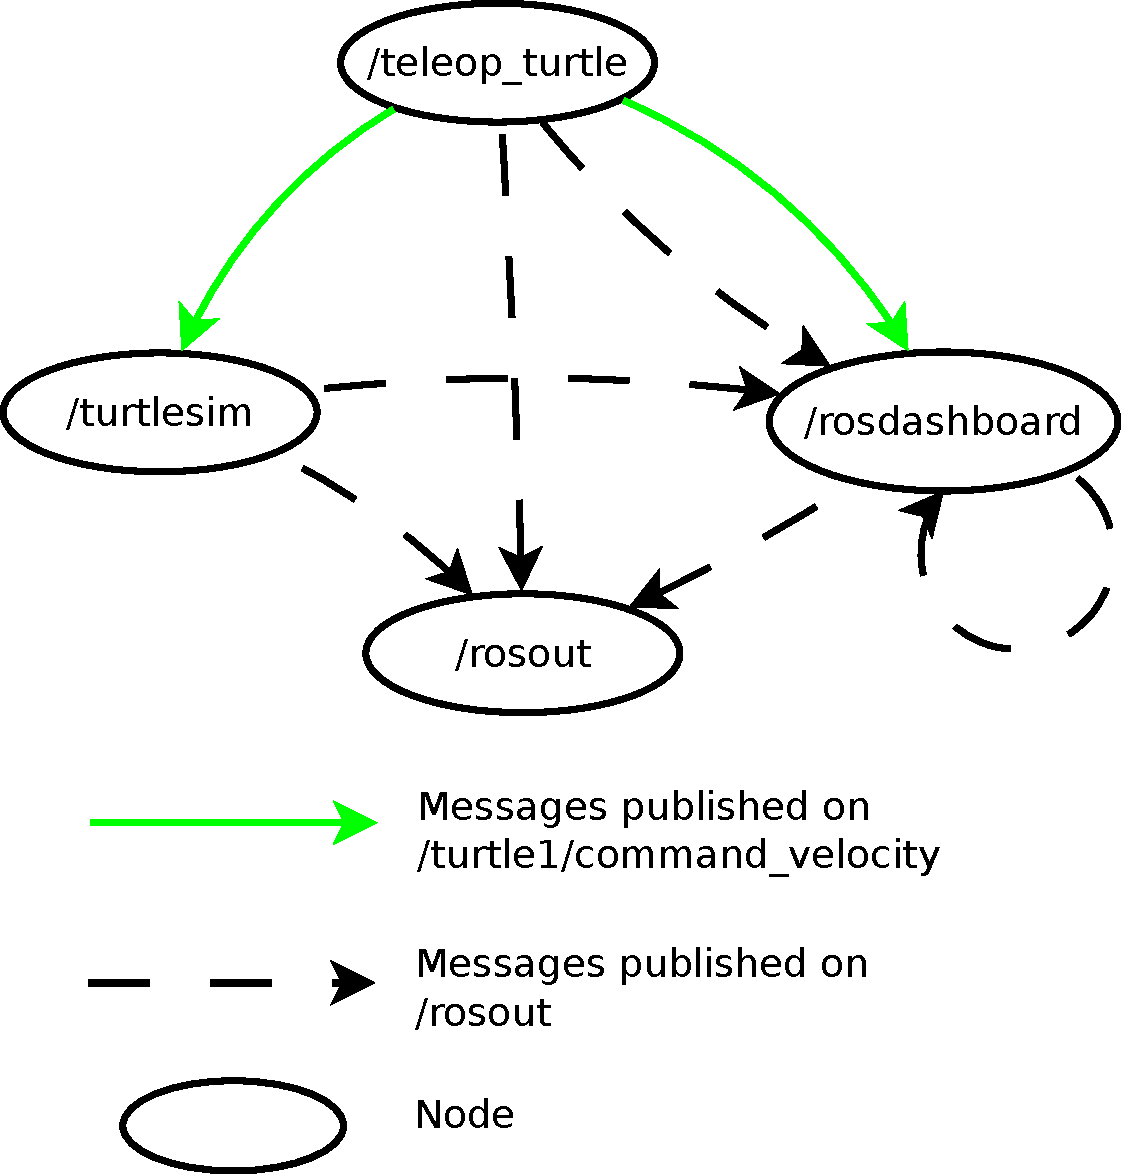
\includegraphics[width=0.7\textwidth]{diagrams/rosgraph}
  }  
  \caption{Simplified ROS computation graph with ROSDashboard.}
  \label{rosgraph_simple}
\end{figure}

\section{Adding New Widgets}
\todo{this could be a good spot for the section from the previous chapter about the plot widget}

\section{NAO Showcase}
A recent problem during the development of an existing project was chosen as use case \comm{showcase? case study?} to evaluate \q the use of ROSDashboard during the debugging of a robot. The project's goal is to use the NAO humanoid robot together with ROS to follow people and engage in conversations with them.

The NAO is a humanoid robot developed and sold by Aldebaran-Robotics\footnote{\url{http://www.aldebaran-robotics.com/}} \cite{Gouaillier2008}. Figure~\ref{nao_coffee} shows an image of the NAO robot used during this case study. The robot comes with a comprehensive list of high level software modules that can be used: a text-to-speech module, a voice recognition module, a walking engine, sound localization, etc. Developers also have access to low level sensor information and can control the actuators directly. The robot is shipped with Choreographe, a graphical programming interface to combine the high level modules to behaviours and create new behaviours.

\begin{figure}[htpb]
  \centering
  \framebox{
    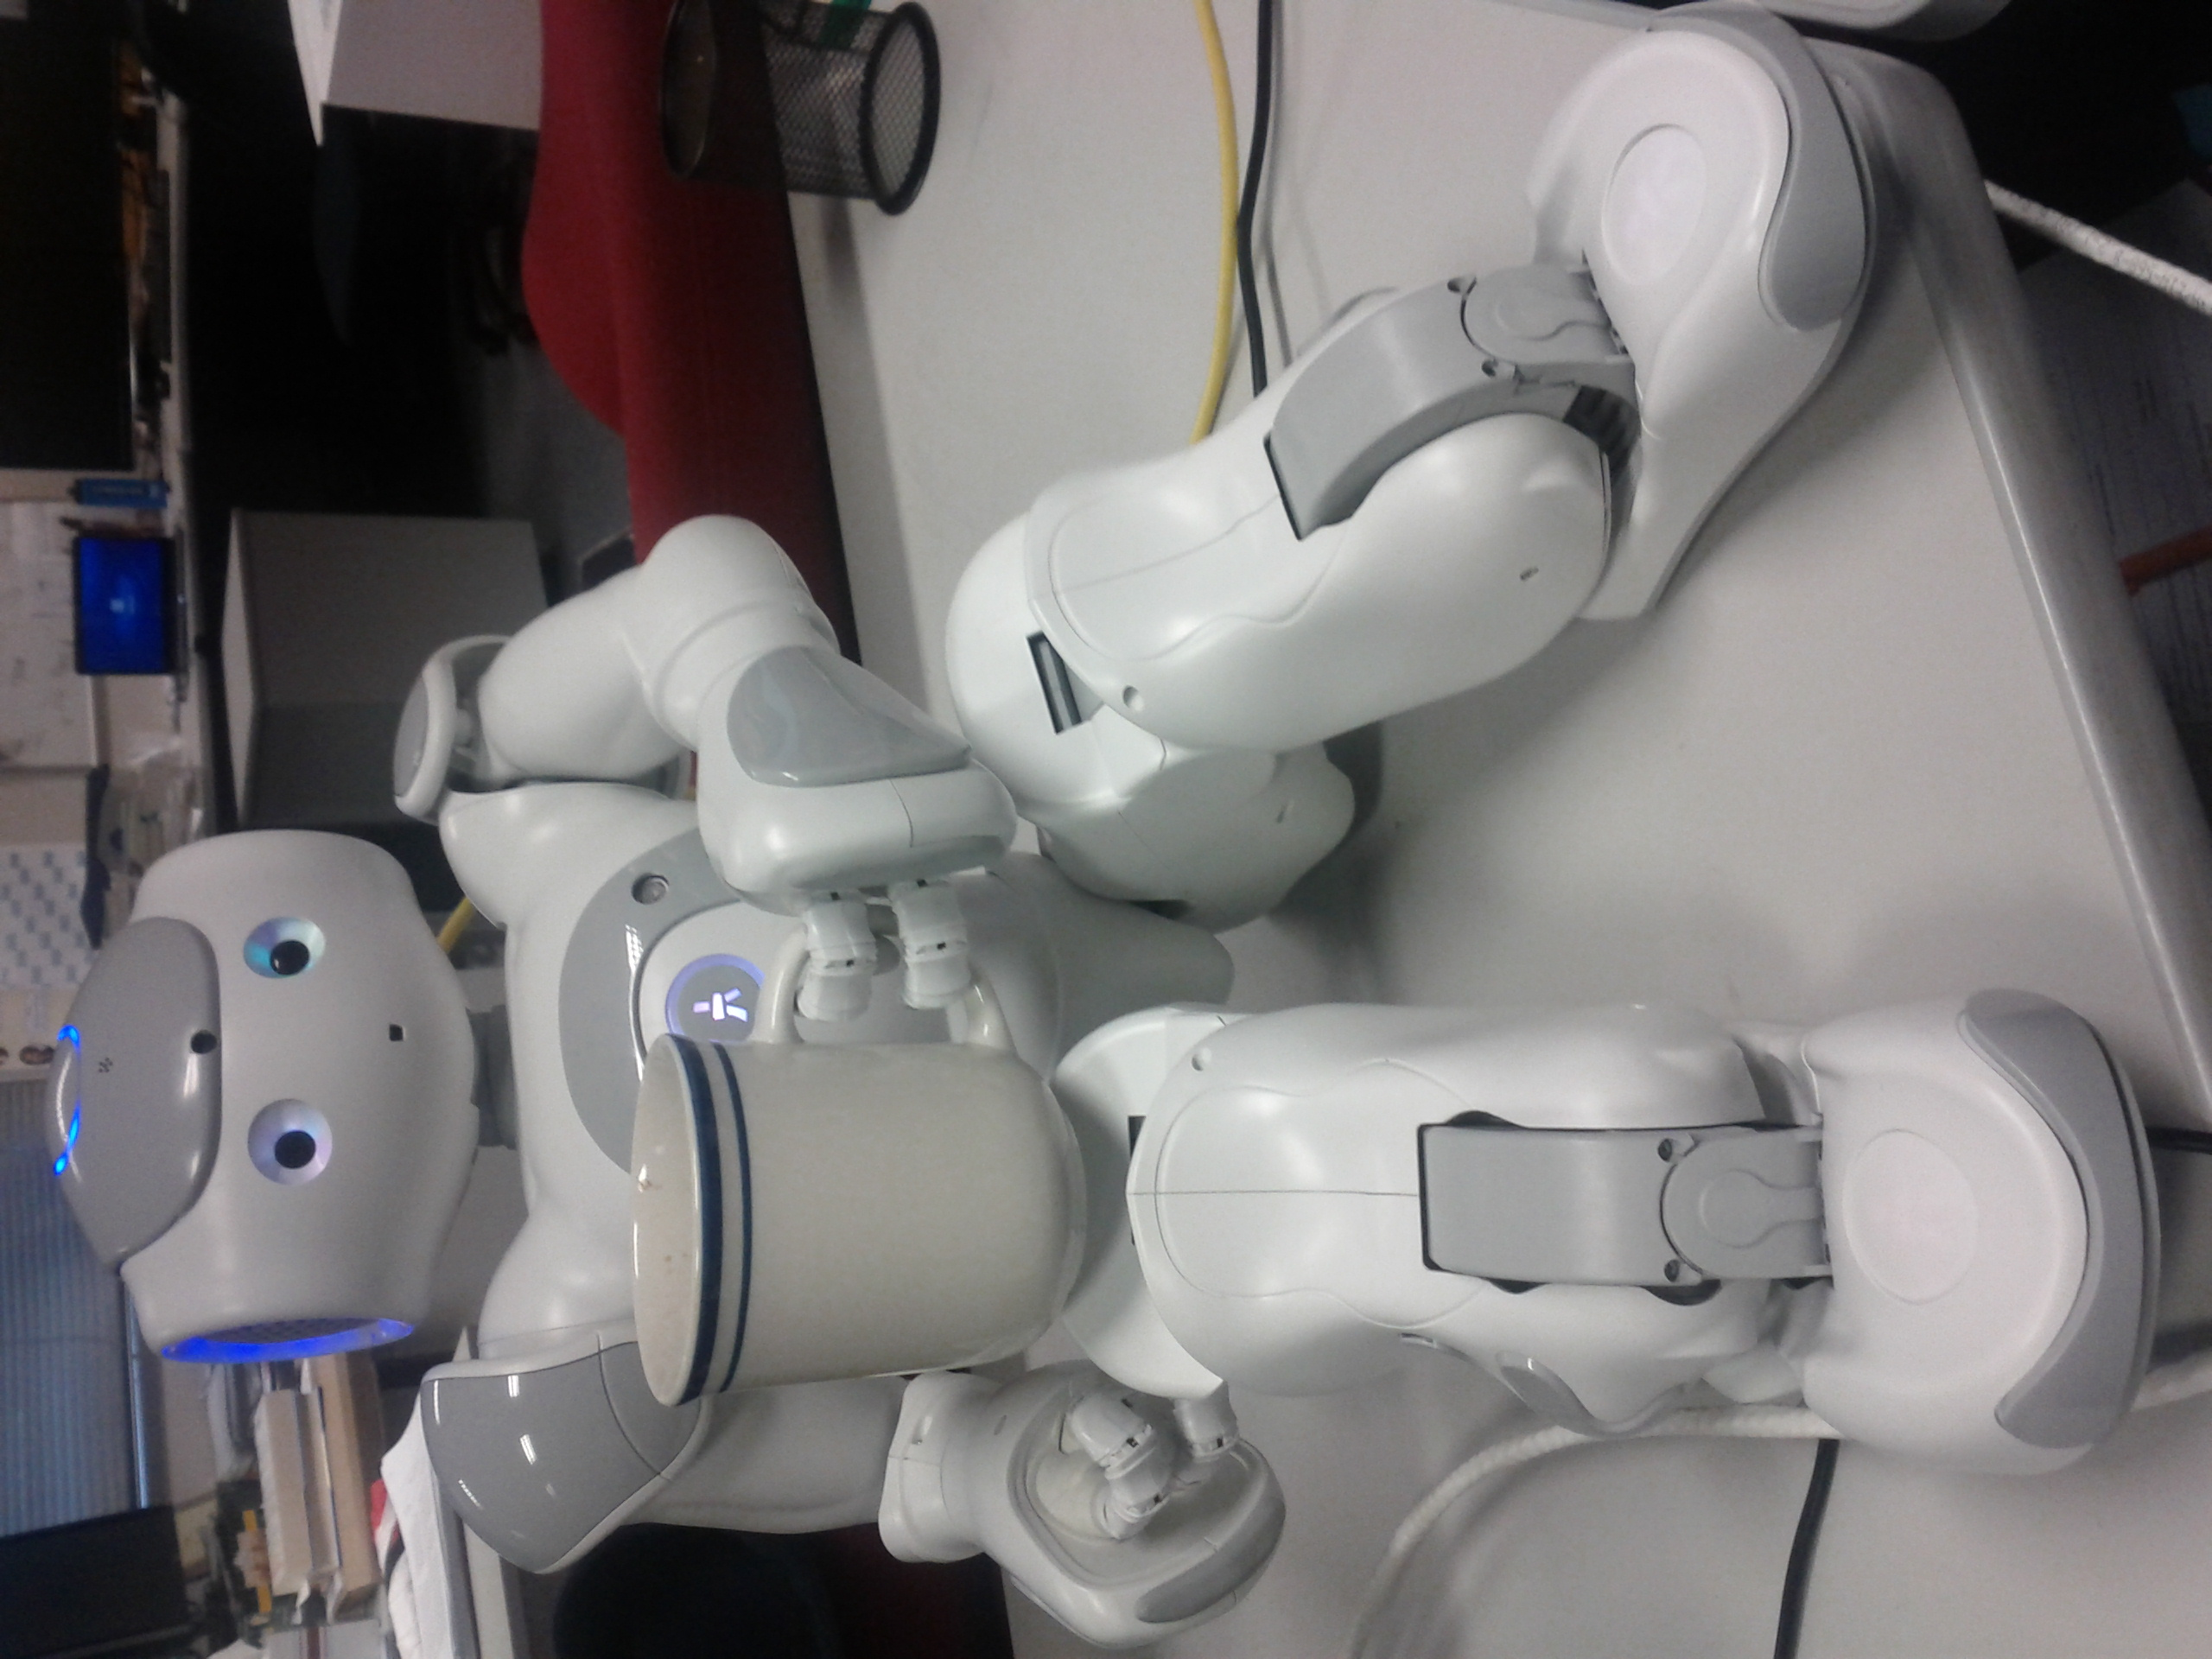
\includegraphics[angle=270,width=0.4\textwidth]{img/nao_coffee.jpg}
  }  
  \caption{NAO robot during the case study.}
  \label{nao_coffee}
\end{figure}

In the project targeted for this case study the sound localization modules was used to move the head towards the person talking to the NAO robot. The sound localization algorithm is part of the SDK and can be accessed through the robot drivers in ROS, which publish the estimated position of a sound source to a topic. The algorithm publishes the location where the sound comes from as a triplet of the horizontal location (azimuth), vertical location (elevation) and confidence. During the initial experiments with the "Sound Tracker" module in Choreographe it seemed like the NAO robot would sometimes point the head to a random direction unrelated to the real direction of the sound source.

The developer of this system tried to find out whether the problem lies with the accuracy of the sensor, the implementation of the sound localization algorithm or the "Sound Tracker" module moving the head. Since the data from the sound source is published as a triplet of numbers, debugging the issue by looking at numbers in a console was challenging. ROSDashboard was used to visualize the values from the sound localization algorithm to determine where the problem of wrong head positions lies.

This section first presents the experimental setup of the case study with the NAO robot. The second part explains how the experiments were conducted with the NAO robot and ROSDashboard, which leads to the results in the third part of this section.

\subsection{Case Study Configuration}
The set up during this case study was distributed on three different machines. The NAO robot has runs a built in Linux which communicated with the master node where the ROS core, Choreographe and the NAO drivers were running. The third machine was a laptop running ROSDashboard and connecting to the respective ROS topics over the network. All three machines were connected to a router by cable. The master node and the laptop with ROSDashboard were both running with Ubuntu 12.04 (64bit) and had the latest ROS release, ROS Fuerte.

While the robot was operated directly by Choreographe, a ROS node was executed as part of the NAO drivers for ROS which published the three values from the sound localization algorithm on the \emph{/sound\_source} ROS topic. The data from this topic was visualized in ROSDashboard. A compass widget was used to visualize the azimuth value from the localization algorithm which represents the horizontal location of the sound source. Since the data published by the localization algorithm is in radiants, it first had to be transformed into degrees for better visualization. Apart from the compass widget a dial was used to visualize the raw radiant value from the algorithm. The confidence of the visualized value was also visualized, a thermo widget was used to display a vertical bar ranging from zero to one. Figure~\ref{nao_dashboard_screenshot} shows the configuration of widgets during the case study, which is also available in the JSON representation in Listing~\ref{nao_dashboard_file}.

\begin{figure}[htpb]
  \centering
  \framebox{
    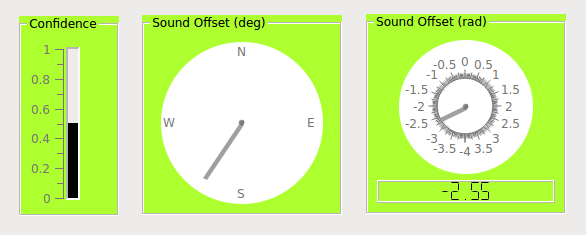
\includegraphics[width=0.9\textwidth]{img/nao_dashboard_screenshot.png}
  }  
  \caption{Widget configuration during the NAO case study.}
  \label{nao_dashboard_screenshot}
\end{figure}

\subsection{Experiments}
To understand what the values from the sound localization algorithm meant a series of tests were conducted. Several sound sources have were created by clapping in close proximity to the NAO robot or simply by talking towards the robot. The first set of test were done with an activated "Sound Tracker" module in Choreographe, which in result moved the head immediately once the NAO robot detected a sound source with a confidence above a certain threshold. The second set of test was conducted without the "Sound Tracker" module. First visualizations of the azimuth value were misleading, but during the case study it became obvious that the position of the sound source is calculated relative to the position of the head and not relative to the position of the body of the robot which was fixed during the case study. Further research showed that the microphones used to determine the location of the sound source are all positioned on the head of the NAO robot.

The tests performed during the case study also showed that the sound localization algorithm usually detects the location of the sound source correctly, but while the head is moved to the desired position more readings came in from the algorithm. These estimated positions were most of the times less confident than the initial sound localization. If the threshold to move the head was set too low, the robot was interrupted during the movement of the head to the position estimated at first and moved the head to a different position. This made the head movement seem random and not related to the actual source of the sound, which was the original problem examined in this case study.

\subsection{Results}
This case study is based on a existing problem that happened during the development of a small but real life robotics project. ROSDashboard was successfully used to visualize data and helped to understand the data published by the sound localization algorithm. In general it also contributed to a better understanding of the robot under development. The data published by the localization algorithm is hard to understand only by looking at the numbers scrolling down in a console. Figure~\ref{comparison} shows the dashboard interface on the left and the raw output collected with the command line tool \verb+'rostopic echo /sound_source'+ in the console. The numbers published by the localization algorithm are representative for most of the data handled during debugging in robotics.

\begin{figure}[ht]
\centering
\subfigure[ROSDashboard]{
    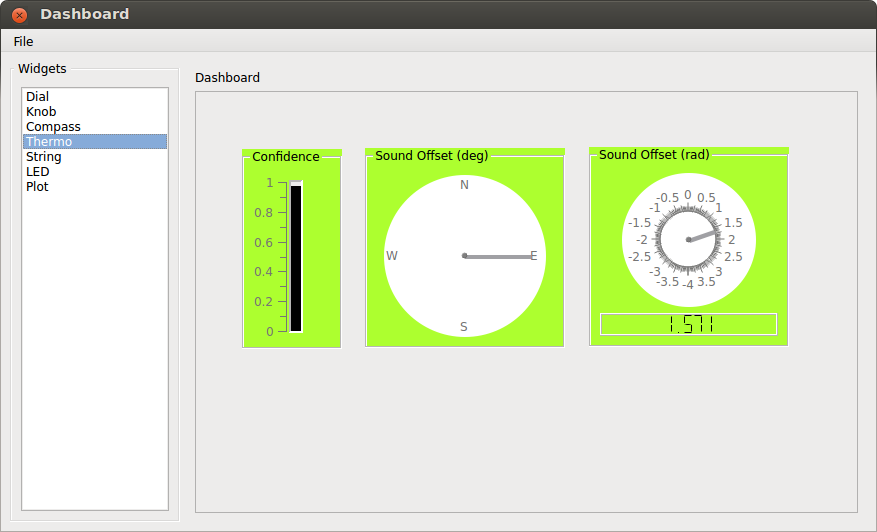
\includegraphics[width=0.9\textwidth]{img/nao_experiment_rosdashboard.png}
}
\subfigure[Console]{
    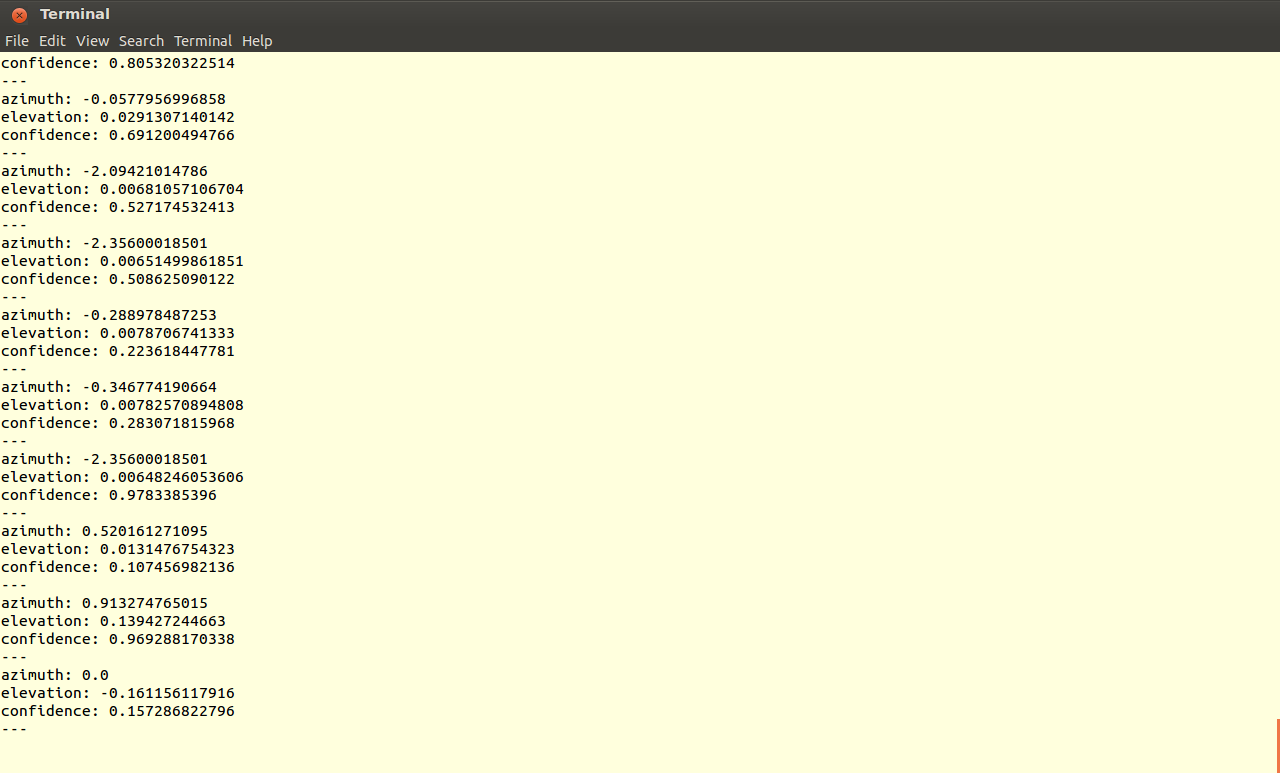
\includegraphics[width=0.9\textwidth]{img/nao_experiment_console.png}
}
\caption{Side by side comparison of ROSDashboard and console output during the case study.}
\label{comparison}
\end{figure}
